\documentclass[11pt,twoside,a4paper]{mpreport}
\usepackage[utf8]{inputenc}
\usepackage[ngerman]{babel}
%\usepackage{a4wide}
%\usepackage[T1]{fontenc}
%\usepackage{textcomp}
%\usepackage{mathptmx}
\usepackage[scaled=0.85]{helvet}
%\usepackage{courier}           % if you really want to use Courier
%\usepackage{url}
\usepackage{cite}
\usepackage{tabularx}
\usepackage{amsmath}
\usepackage{amssymb}
\usepackage[ 
   colorlinks,        % Links ohne Umrandungen in zu wählender Farbe 
   linkcolor=black,   % Farbe interner Verweise 
   filecolor=black,   % Farbe externer Verweise 
   citecolor=black    % Farbe von Zitaten 
]{hyperref}
\usepackage{ngerman}
\usepackage{textcomp}
\usepackage{wdok-title}
\usepackage{tikz,pgfplots}
\usepackage[section]{placeins} 
\usepackage{gnuplottex}
\usepackage{here} 
\usetikzlibrary{patterns}
\usetikzlibrary{fpu}
%%\usepackage[pdf]{pstricks}
\setlength{\parindent}{0pt}
\newcommand{\arcosh}{\mbox{arcosh }}
\pgfplotsset{compat=1.9}
\definecolor{lila}{rgb}{0,0.2,0.8}

% Examples for the definition of convenience commands
\newcommand{\package}[1]{\texttt{#1}}
\newcommand{\foreign}[1]{\emph{#1}}
\newcommand{\q}[1]{»#1«}

% Scale Courier by 0.9
% cf. <http://groups.google.de/groups?selm=yfid76obspu.fsf@triumf.ca>
%\DeclareFontFamily{T1}{pcr}{}
%\DeclareFontShape{T1}{pcr}{m}{n}{
%   <-> s*[.9]pcrr8t
%}{}

\title{Hardware/Software Codesign}
\author{Julian-Benedikt Scholle}
\supervisor{Dr. Ing. Sebastian Zug\\
  Dipl.-Inform Christoph Steup}

\begin{document}
\maketitle
\tableofcontents

\chapter{Einleitung}


\chapter{Das Auto}


\chapter{Anforderungsanalyse}

\section{Ausgangssituation}
Die Ausgangsposition der Arbeit stell sich folgendermaßen dar. Das Fahrzeug basiert auf einem Fahrgestell vom Typ ``Tamiya TT-01-Type E'', welches bereits über einen Motor und einem Motortreiber verfügt.
Auf Grund der Herkunft der Komponenten, dem Modellbau, ist keine
Dokumentation der elektrischen Komponenten verfügbar.
Aus diesem Grund kann der originale Motortreiber nicht verwendet werden.
Da das Fahrzeug über bereits vorhandene 4-Zellen-Lithium-Polymer-Akkus (14,4V Nennspannung) versorgt werden soll um die Anschaffung teurer Akkus zu vermeiden,
hätte dieser so oder so nicht verwendet werden können. 
Für das Fahrzeug wurde bereits eine Treiberplatine in Form eins Prototyps gefertigt.
Diese verfügt über ein Crumb123 Mikrocontroller Modul (At90can128), welches einen Motortreiber vom Typ ``L298 DUAL FULL-BRIDGE DRIVER'' ansteuert.
Des Weiteren verfügt der Prototyp über einen \SI{3}{\A} Schaltregler von Texas Instruments, welcher Mikrocontroller und zwei Pandaboards mit Energie versorgt. 
Der Schaltregler befindet sich durch den Betrieb zweier Pandaboards jedoch bereits an seiner Leistungsgrenze, da ursprünglich nur der Bertieb eines Pandaboards
vorgesehen war. Der verwendete Motortreiber wurde genutzt, da er durch die Verwendung in anderen Projekten bereits vorhanden war, jedoch ist dieser 
nur für Ströme von bis zu \SI{4}{\A} ausgelegt \cite{L298}. In einem Versuch wurden für den im Fahrzeug vorhandenen Motor Ströme von bis zu \SI{20}{\A} gemessen. 
Durch die Unterdimensionierung des Treibers überhitzt dieser bereits nach wenigen Minuten Fahrbetrieb.
Da der vorhandene Motor jedoch weiter verwendet werden soll, muss hier ein leistungsfähiger Ersatz 
entwickelt werden. Des Weiteren fehlen dem Prototyp wichtige Anschlüsse für weitere Sensoren und Beleuchtung, welche nun integriert werden sollen. 

Bei der Entwicklung der neuen Treiberplatine sollen, um Kosten zu sparen, möglichst viele vorhandene Komponenten verwendet werden. Dazu gehören
Microcontroller vom Typ ``Atmel At90can128'', welche in großer Stückzahl vorhanden sind. Benötigte Sensoren in Form eines Interialsensors (Sparkfun SEN-10724)
und Sharp GP2D Sensoren werden ebenfalls vom Lehrstuhl zur Verfügung gestellt. Des Weiteren sind Sortimente von SMD Widerständen und
Kondensatoren in der Größe 805 vorhanden, sodass diese Bauform bei der Entwicklung der Platine bevorzugt wird.

\section{Anforderungen laut Regelwerk}
Um am „Carolo-Cup“ teilnehmen zu können ist ein regelkonformes Fahrzeug nötig, weshalb nun ein Auszug aus den Anforderungen an das Fahrzeug kurz 
aufgelistet und ausgewertet wird.
Alle Anforderungen können im Regelwerk des „Carolo-Cup“ nachgelesen werden \cite{website-carolo-cup-regelwerk}


\subsection{Fahrzeugantrieb und Energieversorgung}
Laut Regelwerk sind alle Teams zur Verwendung eines elektrischen Antriebs verpflichtet.
Die Anzahl der angetriebenen Räder ist nicht vorgeschrieben.
Des Weiteren muss das Auto durch Akkus mit Strom versorgt werden.
Die Übertragung von Daten ist während der Dauer der Disziplinen nicht gestattet

\subsection{Fahrzeugantrieb und Energieversorgung}
Es ist eine Zweiradlenkung der Vorderachse vorzusehen. Die übrige Gestaltung des Fahrwerks bleibt den Teams überlassen. Als
technische Ausprägung ist ausschließlich die Achsschenkellenkung zugelassen.

\subsection{RC-Modus}
In Notsituationen muss es möglich sein das Fahrzeug mit Hilfe einer Funkfernbedienung anzuhalten und manuell zu steuern. Eine solche Notsituation tritt ein, wenn
das Auto seine Aufgabe aufgrund eines Fahrfehlers oder anderem Fehlverhalten nicht mehr autonom fortführen kann.
Der RC-Modus muss per Fernbedienung eingeschaltet und ausgeschaltet werden, bei Aktivierung des RC-Modus muss das Fahrzeug unverzüglich angehalten werden.
Während des Wettbewerbs darf die Geschwindigkeit des Autos $0,3\frac{m}{s}$ nicht überschreiten.
Da das 2,4-GHz Band bereits durch die Vor Ort genutzte Kameratechnik belegt ist, können diese Frequenzen nicht für den RC-Modus genutzt werden.
Der RC-Modus muss durch eine blaue Leuchte an der höchsten Stelle des Fahrzeuges angezeigt werden, welche mit einer Frequenz von 1-Hz blinkt.

\subsection{Signalleuchten}
Durch die Anlehnung des Wettbewerbes an den realen Straßenverkehr muss das Auto über alle in echten Autos vorhandene Signalleuchten besitzen. 
Dazu gehören drei rote Bremslichter am Heck des Autos, sowie jeweils zwei gelbe Blinker rechts und links am Fahrzeug. Die Blinkfrequenz der Blinker muss
1-Hz betragen.

\section{Auswertung des Regelwerks}
Der vorhandene Prototyp entspricht bereit den Anforderungen bezüglich des elektrischen Antriebs, jedoch mit den bereits beschriebenen Unzulänglichkeiten. 
Um diese Unzulänglichkeiten zu korrigieren, muss ein leistungsfähiger Motortreiber integriert werden.
Die Lenkung des Autos kann von einem einfachen Servomotor vorgenommen werden. Ein solcher wurde bereits in Form eines IQ-620CMG des Herstellers Hype angeschafft. 
Damit das Auto die im RC-Modus nötigen Funksignale auswerten kann, muss ein Empfänger integriert werden. Dieser wird jedoch über USB zur Verfügung gestellt
und ist deswegen nicht Teil dieser Arbeit. Des Weiteren muss das Auto mit den nötigen Signalleuchten ausgestattet sein, dazu gehören Blinker rechts und links
jeweils vorne und hinten, sowie drei Bremsleuchten an der Rückseite und eine weitere Leuchte welche den RC-Modus anzeigt. Der Vollständigkeit halber kommt hier noch die
Frontbeleuchtung hinzu.

\section{Andere Anforderungen}
\subsection{Anforderungen durch Bewertungskriterien}
Abseits des Regelwerkes ergeben sich weitere Anforderungen durch die Bewertungskriterien des Wettbewerbes. Dabei handelt es sich um nichtfunktionale Anforderungen.
So muss das Team während der statischen Disziplinen ihr Gesamtkonzept präsentieren. Schwerpunkte dabei sind, Hardware- und Software-Architektur sowie Energiebedarf und 
Herstellungskosten \cite{website-carolo-cup-regelwerk}. Daraus entstehen weitere Anforderungen: Energieeffizienz und Herstellungskosten. \\


\subsection{externe Anforderungen}
Folgende Anforderungen werden durch das Team an die Platine gestellt. Die Integration einer Inertialsensorik (Sparkfun SEN-10724) zur Inertialnavigation,
Anschlüsse Infarotsensoren vom Typ Sharp GP2D120 und GP2D1202, die Integration einer Odometrie zur Geschwindigkeitsmessung,
sowie eine 5V Stromversorgung zum Betreiben eines Pandaboards. Die Platine soll ein ROS-Interface auf einem Pandaboard zur Verfügung stellen, mit welchem die Aktorik gesteuert und
die Sensorwerte ausgelesen werden können. Das Auto soll über ein vorhandenes Netzteil betrieben werden können (ca. 20V).

\section{Zusammenfassung}
Um den Anforderungen zu genügen, muss ein Motorteiber mit einer Belastbarkeit von mindestens 20 Ampere integriert werden. 
Ein Mikrocontroller zum Steuern der Aktorik inklusive des Motors, sowie zum Auslesen der Sensorsignale muss zur Verfügung gestellt werden. 
Anschlüsse für zwei Sharp Sensoren vom Typ ``GP2D120'' oder ``GP2D12'' sowie weitere Anschlüsse für den Inertialsensor, Beleuchtung, Servomotor werden ebenfalls benötigt. 
Es muss eine Odometrie zur Messung der Geschwindigkeit integriert werden.
Es muss eine effiziente Energieversorgung aller Bauteile zur Verfügung gestellt werden, welche auch zwei Pandaboards stabil betreiben kann. Die maximale Eingangsspannung
muss mindestens 20 Volt betragen um das Auto auch über das Netzteil betreiben zu können.
Da das Fahrzeug energieeffizient arbeiten soll, ist eine Messung des Motorstromverbrauches essenziell um das Fahrverhalten bezüglich der Effizienz bewerten zu können.
Zu guter Letzt muss die Platine über eine Schnittstelle mit einem Pandaboard kommunizieren und seine Daten dort über ein ROS-Interface zur Verfügung zu stellen.

\section{Änderung der Anforderungen}
Nach der erfolgreichen Teilnahme am ``Carolo-Cup Junior'' im Februar 2014, begann die Weiterentwicklung des Konzepts. Während der Entwicklung kamen jedoch
einige Flaschenhälse zum Vorschein, sodass in der Projektphase die Hardwareplattform geändert werden musste. Die Rechenleistung der Pandaboards stellte sich
als unzureichend heraus und es wurden mehr Distanzsensoren gewünscht. Die Pandaboards wurden nach der Absprache mit dem Team durch ein Intel NUC vom Typ
D34010WYB ersetzt. Laut Datenblatt \cite{datasheet-nuc} besitzt der NUC einen Weitbereichseingang zur Spannungsversorgung, dieser ist für 12-24 Volt zugelassen.
Sodas der NUC direkt an den 14,4V der Akkus und den 20V des Netzteils betrieben werden kann. Um Verwirrungen zu vermeiden wird im Folgenden legendlich 
von Recheneinheit gesprochen, wenn es nicht relevant ist ob es sich um NUC oder Pandaboard handelt.


\chapter{Stand der Technik}

\chapter{Auslegung der Stromversorgung}

Um das Layout der Platine möglichst simpel zu halten und damit kostengünstig zu bleiben, wurden alle Komponenten so ausgewählt dass diese über eine einzige 5V Spannungsquelle mit Energie versorgt werden können.
Es wichtig den Stromverbrauch aller Komponenten abzuschätzten, um die Spannungsversorgung sinnvoll Dimensionieren zu können. Eine zu schwache spannungsquelle kann zu instabilitäten führen,
während eine überdimmensionierte Geld verschenkt.

\section{Stromverbrauch der Komponenten}
In diesem Abschnitt soll eine Abschätzung des Stromverbrauches vorgenommen werden. Dabei wird keinen Wert auf hohe Genauigkeit gelegt, es soll nur eine ungefäre Größenordnung für den Stromverbrauch gefunden werden.

\subsection{Servomotor}
Der Stromverbrauch des Servomotors ist schwer zu ermitteln, da es sich um einen Modellbauservomotor handelt 
sind im Datenbatt hierzu leider keine Daten aufzufinden. Da ein Messaufbau für die Abschätzung des Stromverbrauches
zu Aufwändig ist, werden hier Messwerte eines ähnlichen Servos aus einem Artikel \cite{website-servo} herangezogen.
Laut diesem hat eine Servomotor keinen konstanten Stromverbrauch. Der Stomfluss wird immerwieder unterbrochen, so das es zu einem Intervallartigen Stromfluss kommt.
Nur wenn der Servomotor dauerhaft belastet wird kommt es zu einem konstanten Stromfluss.
Im Artikel werden mehrere Servomotorn vermessen, der Motor der unserm am nächsten kommt ist der ``Graupner 4421'' mit folgenen Daten:

Technische Daten ``Graupner 4421'' \cite{website-servo-vergleich-dat}:
\begin{itemize}
 \item Stellzeit(60°): 0,11s
 \item Stellmoment: 88Ncm 
\end{itemize}


Technische Daten des verwendeten Servomotors \cite{website-servo-dat}:
\begin{itemize}
 \item Stellzeit(60°): 0,13s (4,8V) / 0,16s (6,0V)
 \item Stellmoment: 92Ncm (4,8V) / 78Ncm (6,0V)
\end{itemize}



Dieser hat laut des Artikels eine maximale Stromaufnahme von 1,2A. Um noch Luft nach oben zu haben wird hier ein Verbrauch von 
1,8A angenommen.

\subsection{Pandaboard ES}
Leider gibt es vom Hersteller des Pandaboards keine konkreten Angaben zum Stromverbrauch. Der Hersteller empfiehlt jedoch ein
Netzteil mit 4A\cite{website-panda-supply}, wobei auch ein Betrieb an USB mit hilfe eines Y-Kabels möglich ist. Die USB-2.0 Spezifikation\cite{website-usb-spec} sieht eine maximale 
Stromabgabe von 500mA vor.

Der Stromvebrauch des normalen Pandaboards (ohne ES) beträgt ca. 800mA \cite{website-panda-power}.
Nähere angaen zu Stromverbrauch des normalen Pandaboards (ohne ES) finden sich in \cite{website-panda-power}.
Der Verbrauchdes Pandaboard ES dürfte durch de Schnelleren Prozessor minimal darüber liegen. 
Durch anschluss von USB Geräten an dasBoard kann der Stomverbrauch jedoch noch steigen, Die USB-Spezifikation \cite{website-usb-spec}
sieht pro Port eine maximale Stomentnahme von 500mA vor. Da das Pandaboard über 2 USB ports verfügt liegt der maximale zusätzliche Verbrauch bei 1A
Sodas hier ein gesammt Verbrauch von 2A veranschalgt wird.

\subsection{Led Beleuchtung}
Auch wenn LEDs den Ruf haben besonders energieffizient zu sein ist der Stromerbrauch beieiner größeren anzahl nicht zu
unterschätzen. Da wir RBG-LEDs einsätzen besteht ein LED-Modul aus 3 LEDs in den Grundfarben rot, blau und grün.
Laut Datenblatt \cite{ds-WS2812} haben die LEDs eine Stromaufnahme von 20mA, also 60mA pro Modul.
Um Reglelwerk konform zu sein, werden folgende Beleuchtungen benötigt: Blinker rechts und links jeweils vorne und hinten.
Sowie eine leuchte welche din RC-Modus anzeigt. Zusätzlich zu denim Reglelwerk vorgeschriebenen Beleuchtungen werden noch
2 Frontscheinwerfer und Rückleuchten integriert. So dass sich eine Anzahl von 9 LED-Modulen ergibt.
Der maximale durch die LEDs verursachte Verbrauch liegt somit bei 540mA. 



Bremslichter???


\subsection{Microkontroller}
Der maximale Stromverbrauch des AVR Mikrocontrollers liegt laut Datenblatt\cite{ds-at90can} bei 200mA, wenn IO-Pins belastet werden
Der Mikrocontrollers selber braucht jedoch bei 5V Betriebsspauung und 16MHz nur 29mA. Da die IO-Pins des Controllers nur wenig belastet werden,
wird hier nur ein Verbrauch von 100mA veranschlagt.

\subsection{Sharp Sensoren}
Die Sharp GP2D120 distanz Sensoren liegt laut Datenblatt \cite{ds-sharp-GP2D120} bei 50mA, da 2 dieser Sensoren verbaut werden ergeben sich 100mA.

\subsection{Sonstige Peripherie}
Da der Stromverbrauch der restliche Komponenten minimal ist werden hier pauschal 100mA veranschalgt.

\section{Auswahl des Reglers}
Der Gesammtstromverbrauch der Komponenten beträgt 4.740mA. Ein Linearregler hier nicht mehr praktikabel, da dieser bei einer Akkuspannung von 14,4V und 3.740mA fast 45 Watt Leistung in Wärme umwandeln würde.
Eine gute Wahl für diesen Einsatzzweck ist der LM2678 von Texas Instruments, dieser kann dauerhaft einen Strom von 5A liefern und sein Wirkungsgrad liegt selbst bei maximallast bei über 80\%.
Eine Übersicht dazu findet sich in Abbildung [\ref{fig:vreg}].
\begin{figure}[H]
\centering
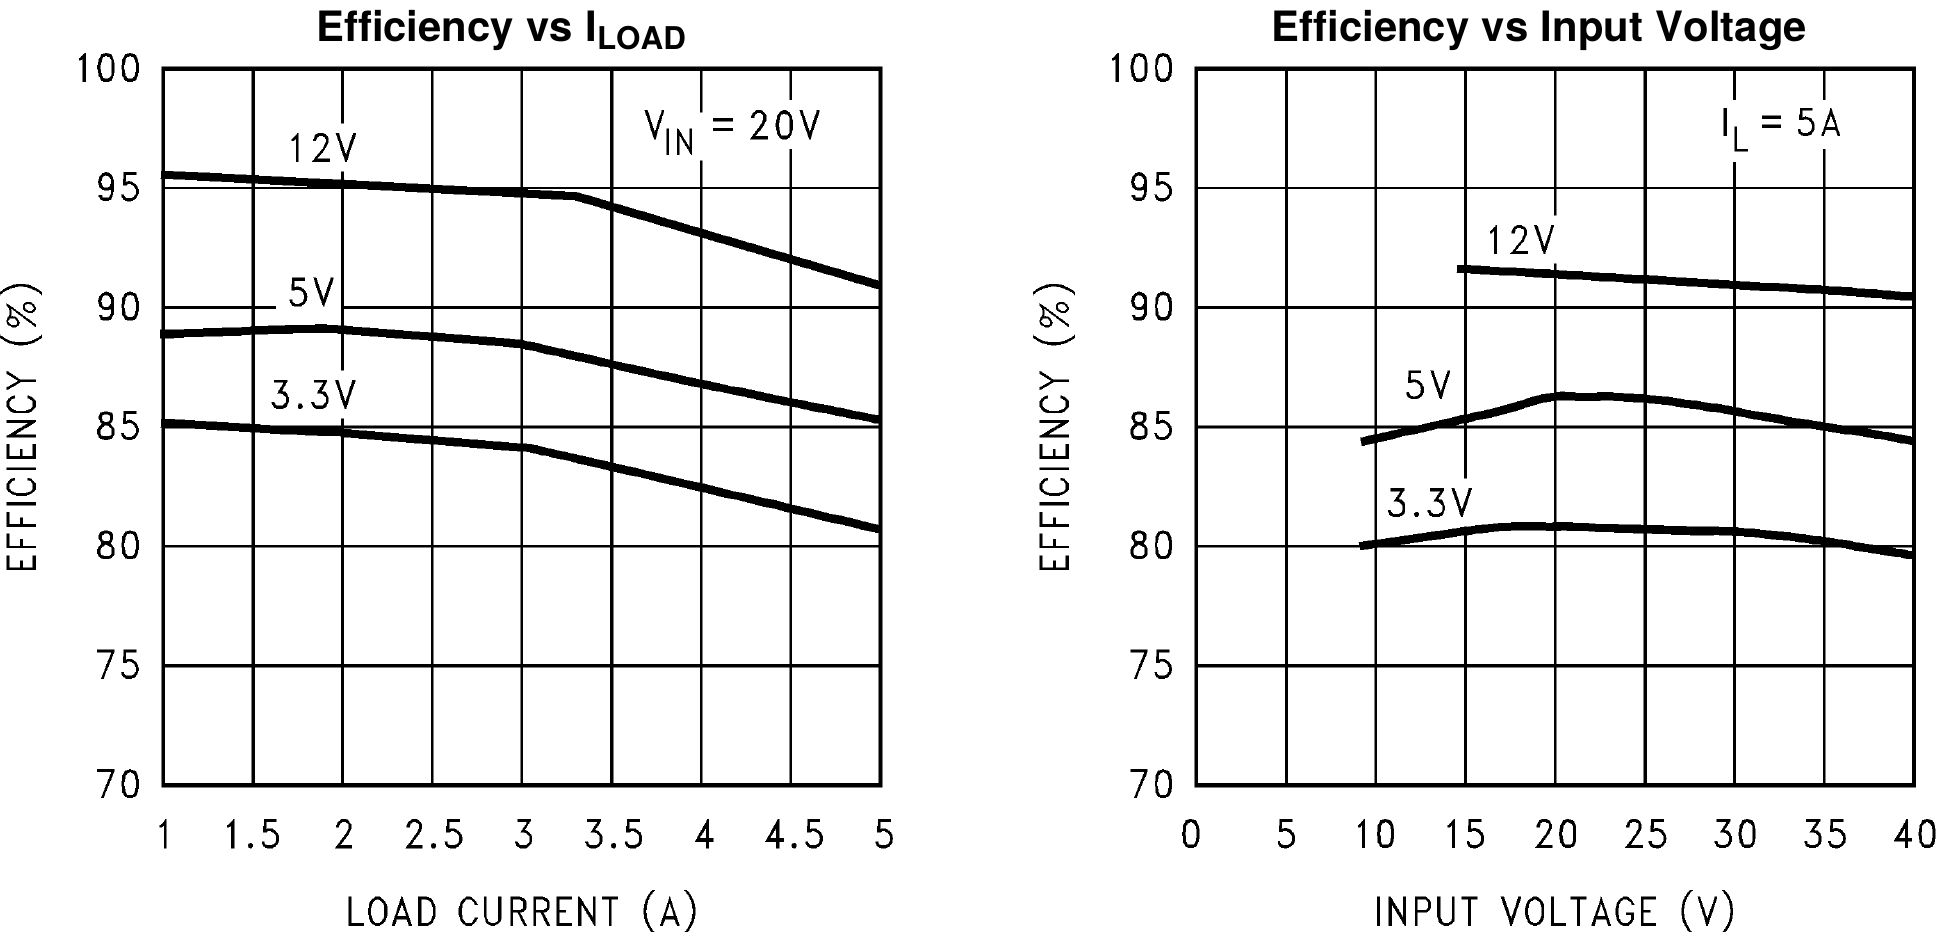
\includegraphics[width=.8\textwidth]{vreg.png}\\
\caption{Regulator Wirkungsgrad}%
\label{fig:vreg}
\end{figure}
Ausgehend von ca. 24 Watt Leistungsaufnahme ($4,8A*5V$) und einem minimalen Wirkungsgrad von 80\%  ergibt sich damit eine überschauliche Verlustleistung von 6 Watt.



\chapter{Motoransteuerung}

\section{Treiberbausteine}
Da die gewählten Akkus eine Spannung von 14,4V aufweisen, kann der orgiginal Motortreib erleider nicht verwendet werden.
Denn dieser benötig eine Spannung von 7,4V. Da der AVR Mikrokontroller mit 5V betrieben wird, wird ein Motorteiber benötig der
mit den 5V Pegeln arbeiten kann. In vielen Mikrocontroller Projekten und in unserem ersten Prototyp wird der L298 DUAL FULL-BRIDGE DRIVER
verwendet. Dieser ist leider auch bei der Benutzung beider Kanäle auf 4 Ampere begrenzt \cite{L298}, was beim Prototy zu einer Permanenten
überlastung des Treibers führt. Leider sind keine vollintegrierten Motortreiber mit der benötigten Belastbarkeit verfügbar.
Um die bentötigte Belastbarkeit zu erreichen wird der zur Ansteuerung benötigte Vierquadrantensteller aus diskreten Mosfets aufgebaut.

\subsection{Vierquadrantensteller}
Definition nach Wikipedia:\\
``Ein Vierquadrantensteller besteht aus einer elektronischen H-Brückenschaltung aus vier Halbleiterschaltern, meist aus Transistoren, 
welche eine Gleichspannung in eine Wechselspannung variabler Frequenz und variabler Pulsbreite umwandeln kann. Vierquadrantensteller 
in der Energietechnik können auch Wechselspannungen unterschiedlicher Frequenzen in beiden Richtungen ineinander umwandeln.''


\begin{figure}[H]
\centering
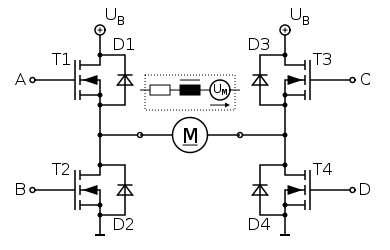
\includegraphics[width=.8\textwidth]{Vierquadrantensteller.png}\\
\caption{Vierquadrantensteller}%
\label{fig:Vierquadrantensteller}
\end{figure}


Auf Grund der hohen Belastbarkeit werden meißt Mosfets als Halbleiterschalter genutzt. Um die beiden oberen Mosfets (T1/T3) durchzuschalten
ist auf Grund des fehlenden Massepotentials eine Gatespannung oberhalb der Betriebsspannung nötig. Diese wird meist mittels Bootstrapping zur
Verfügung gestellt. Da das Simultane durch schalten der Übereinander liegenden Mosfets zu einem Kurzschluss führen würde, muss dies durch
eine Schutzschalung verhindert werden. Um all diese Funktionen zur verfügung zu stellen gibt es bereits fertige Mosfettreiber Bausteine,
was dass Schaltungsdesign enorm vereinfacht.

\section{Mosfettreiber}
\subsection{Verfügbarkeit}

Mosfettreiber gint es in vielenAusführungen, unter anderem als ``Single Channel High Side Driver``, ``Half Bridge Driver'', ``Full Bridge Driver''
und ``3 Phase Driver''. Da für den Verbauten DC-Motor eine Vollbrücke nötig ist, um den Motro in alle Richtungen zu betreiben, Werden an dieser Stelle
ausschließlich ``Full Bridge Driver'' untersucht.

Eine Tabelle auf Mikrocontroller.net\cite{FET_D_TABLE} zeigt eine Auswahl an verfügbaren Mosfettreibern. Dort sind zwei
``Full Bridge Driver'' aufgeführt, welche für dieses Projekt passend sind. Allerdings fällt die Entscheidung auf einen anderen Treiber,
dem Allegro A3941.
\subsection{Allegro A3941}
Der Allegro A3941 ist f+r Betriebsspannungen von 5,5V bis 50V geeignet und liegt damit in der Spezifikation des Projekts.
Des weiteren verfügt der Motor über eine integrierten 5V Regulator und kann somit ohne Spannungsregulator am Akku betrieben werden.
Über zwei Ausgänge der Treibers können diverse Fehler ausgelesen werden.


Der Treiber lässt sich in verscjiedennenModi betreiben:

\begin{figure}[H]
\centering
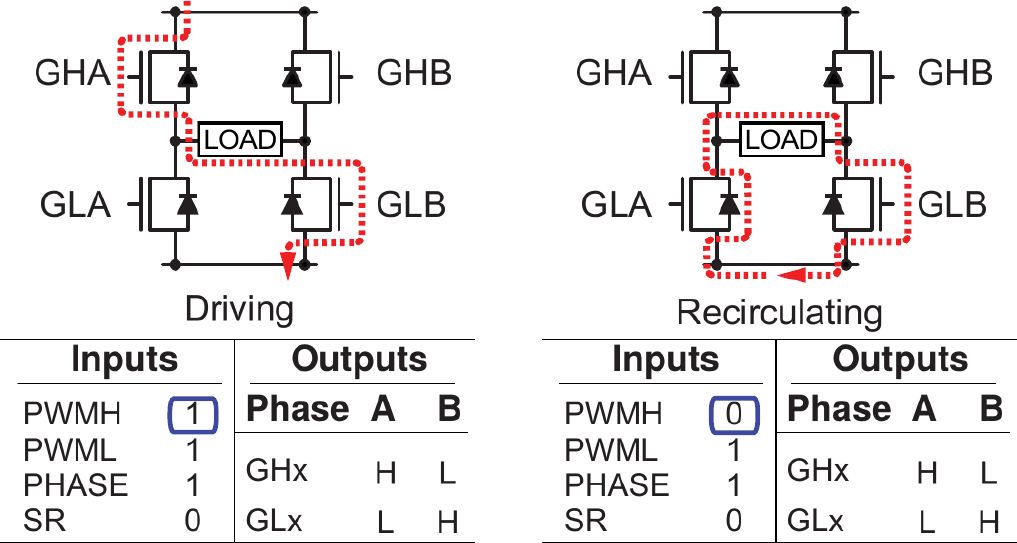
\includegraphics[width=.8\textwidth]{3941_1.png}\\
\caption{Slow decay, diode recirculation, high-side PWM}%
\label{fig:3941_1}
\end{figure}

Konfiguration: PWML=1, PHASE=1, SR=0 und PWM an PWMH (high-side PWM)\\
Bei aktivierten PWMH fließt der Strom durch den GHA-Mosfets über den Motor und
dann über den GLB-Mosfet. in diesem Modus wird der Motor angetrieben.
Wenn PWML deaktiviert ist zirkuliert der vom Motor induziert Strom durch GLB und durch
die interne Diode von GLA, der Motor wird dadurch gebremst.


\begin{figure}[H]
\centering
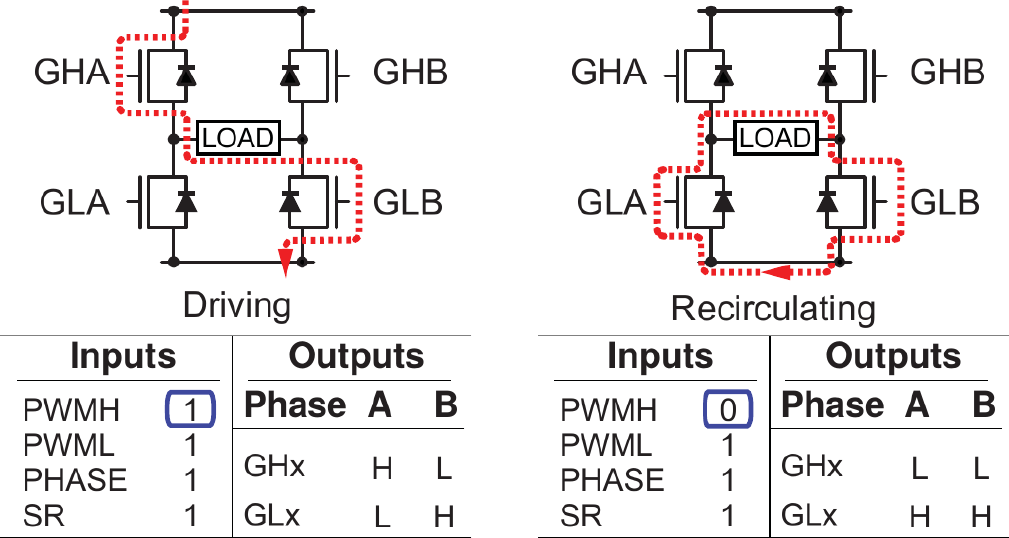
\includegraphics[width=.8\textwidth]{3941_2.png}\\
\caption{Slow decay, SR active, high-side PWM}%
\label{fig:3941_2}
\end{figure}

Konfiguration: PWML=1, PHASE=1, SR=1 und PWM an PWMH (high-side PWM)\\
Bei aktivierten PWMH fließt der Strom durch den GHA-Mosfets über den Motor und
dann über den GLB-Mosfet. in diesem Modus wird der Motor angetrieben.
Wenn PWML deaktiviert ist zirkuliert der vom Motor induziert Strom durch 
GLB und durch GLA, der Motor wird durch den niedrigeren Innenwiederstand des Mosfest 
stärker gebremst als in der Voherigen Konfiguration. Dabei ist darauf zu achten, dass
beinahe die gesamte induzierte Spannung über den beiden Mosfets (GLA/GLB) abfällt.
Was zu einer starken Hitzeentwicklung führen kann.



\begin{figure}[H]
\centering
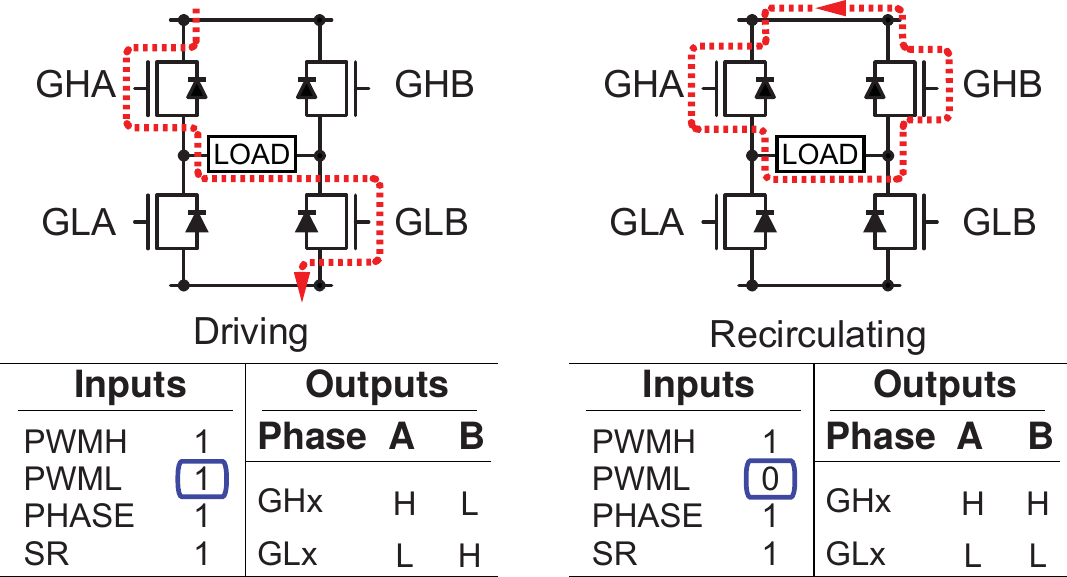
\includegraphics[width=.8\textwidth]{3941_3.png}\\
\caption{Slow decay, SR active, low-side PWM}%
\label{fig:3941_3}
\end{figure}

Konfiguration: PWMH=1, PHASE=1, SR=1 und PWM an PWML (low-side PWM)\\
Diese Konfiguration entspricht im Grunde den beiden vorherigen, Nur das dass PWM-Signal
an den unteren Mosfets anliegt. Der SR-Pin entscheidet wieder darüber ob im ``Bremsmodus''
die internen Dioden genutzt werden (SR=0) oder nicht (SR=1)




\begin{figure}[H]
\centering
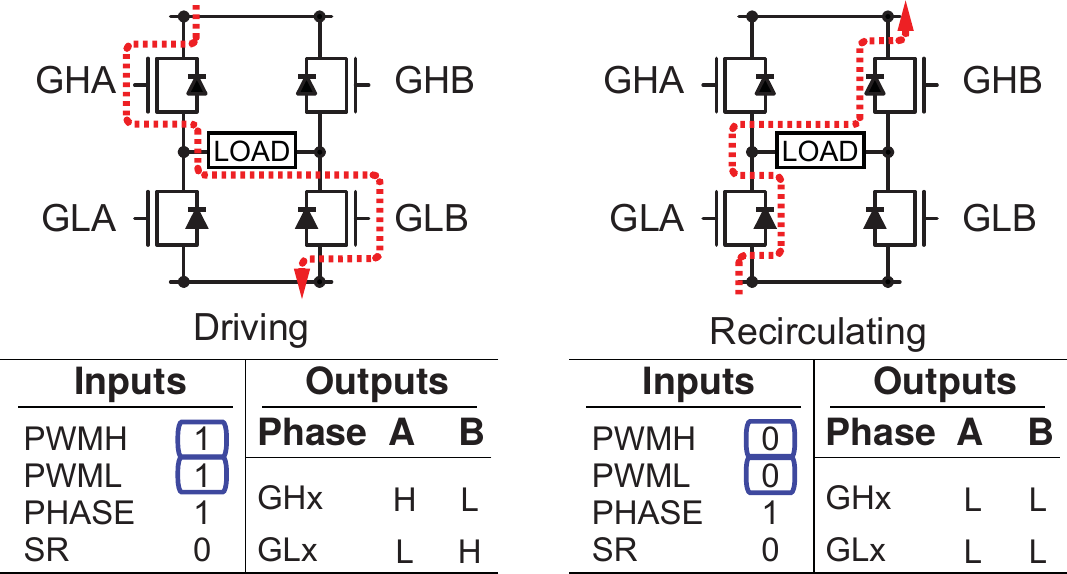
\includegraphics[width=.8\textwidth]{3941_4.png}\\
\caption{Fast decay, diode recirculation}%
\label{fig:3941_4}
\end{figure}


Konfiguration: PWMH=1, PWML=1, PHASE=1, SR=1\\
in dieser Konfiguration werden die oberen und unteren Mosfets gleich geschaltet. Im
``Bremsmodus'' führt das dazu das der induzierte Motorstrom nicht über die Mosfets
zirkulieren kann. Der Strom fließt stattdessen zurück in die Spannungsquelle, was
abhängig von der Spannungsquelle zu Schäden führen kann. Wird die Schaltung jedoch an
einem Akku betrieben ist es so möglich die Energie zu nutzen und damit den Akku
zu laden.

\begin{figure}[H]
\centering
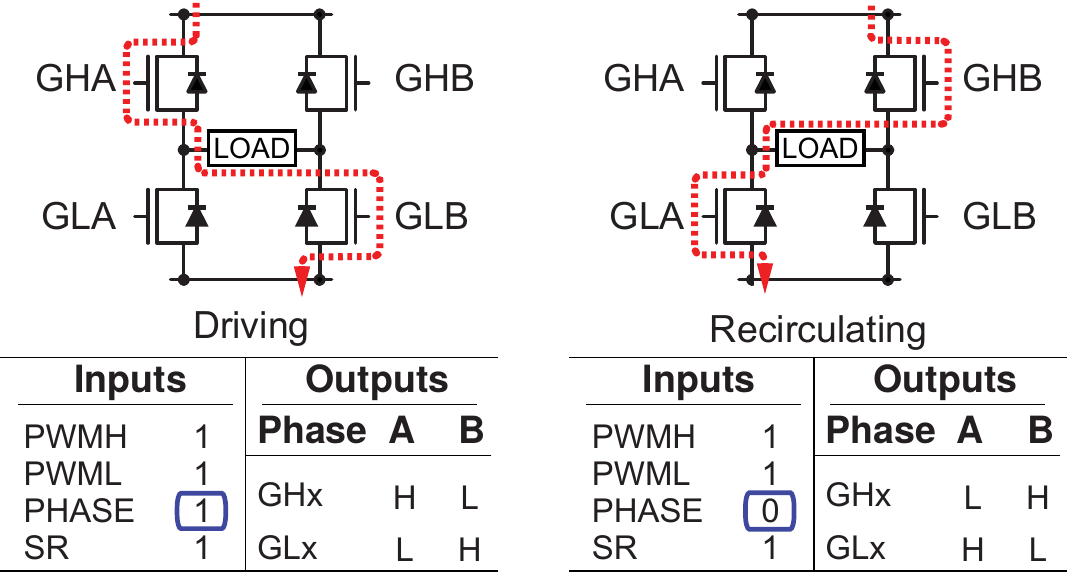
\includegraphics[width=.8\textwidth]{3941_5.png}\\
\caption{Fast decay, SR active, full four-quadrant control}%
\label{fig:3941_5}
\end{figure}

Diese Konfiguration zeigt den Einfluss des PHASE-Pins. Liegt am PHASE-Pin 1 ein an
fließt der Strom von links nach rechts. Liegt 0 an fließt er von rechts nach links.
Mithilfe des PHASE-Pins wird also die Polung des Motors festgelegt.



\chapter{Motorstrommessung am Shunt}


\section{Problem}

An einem mit PWM angesteuertem DC-Motor soll eine Strommessung mit Hilfe eines Shuntwiederstandes
durchgeführt werden. Aufgrund der PWM Ansteuerung muss der DC-Anteil aus dem Signal herausgefiltert werden!


\section{Prinzip der Strommessung}

Die Messspannung wird über einen Shuntwiederstand zur Masse gemessen! Aufgrund nicht vorhandener Datenblätter des Motors
wird von einem expirimentel Ermittelten maximalen Strom des Motors ausgegangen. Dieser beträgt bei einer Betriebsspannung von 20V ca. 20A.
Da einen Shunt mit einer maximalen Belastbarkeit von 2 Watt eingesetzt wird, darf der maximale Spannungsabfall am Shunt 100mV nicht überschreiten.
Nach dem Ohmschen Gesetz ergibt sich dadurch ein Widerstand von $0,005 \Omega$  für den Shunt. Shuntwiederstände in der Größe sind problemlos zu bekommen.
Da es sich hier um eine Worst Case Rechnung handelt, wird der zusätzliche Widerstand des Shuntwiederstandes und der damit verringerte Strom bewusst ignoriert.

Die über den Shuntwiederstand gemessene Spannung soll über den ADC Eingang des Mikrocontrollers eingelesen werden. Vorher jedoch muss das Signal gefiltert werden, da der Strom
durch die Ansteuerung mittels der Pulsweitenmodulation nicht konstant ist!



\section{Anforderungen}
Die maximale Auflösung des Mikrocontrollers soll ausgenutzt werden. Der ADC des Mikrocontrollers arbeitet mit einer Auflösung von 10 Bit und einer 
Referenzspannung von 5V. Um die Auflösung des ADC auszunutzen muss das Signal, aufgrund unseres Spannungsabfalls verstärkt werden.

Als Anforderung ergibt sich außerdem, dass der maximale Ripple des Endsignals kleiner ist als der Quantisierungsfehler des ADC.
So ist es möglich aufeine zusätzliche digitale Filterung weitgehend zu verzichten.
Die kleinst mögliche zu erfassende Spannung des ADC beträgt $\frac{5}{2^{10}}=4,88mV$.
Diesen wert sollte der Ripple des Endsignales nicht überschreiten.
Aus einem möglichst kleinem Ripple resultiert eine möglichst hohe Filterordnung bzw. eine niedrige Grenzfrequenz.
Allerdings soll $U_{DC}$ einer Änderung des Mittelwertes, also einer Änderung des Tastverhältnisses, möglichst
schnell folgen. Diese Anforderung widerspricht der Vorherigen, so das ein Kompromiss gefunden werden muss.

\section{Bestimmung des Filtertyps}
Aufgrund des sehr niedrigen Spannungspegels am Shunt,ist es nötig das Signal zu verstärken. Da zum verstärken des Signals aktive elektronische Elemente notwendig sind,
z.B. ein Operationsverstärker, wird an dieser Stelle gleich ein aktiver Filter verwendet. Dieser gibt uns die Möglichkeit des Messignal zu verstärken und gleichzeitig zu
Filtern. Da wir als unser Signal im optimalen Fall eine Gleichspannung darstellt müssen wir die Hochfrequenten Anteile unseres Signales herausfiltern, dies geschieht 
mit Hilfe eines Tiefpasses. Es gibt im Grunde 2 übliche aktive Tiefpässe, den Tiefpass mit Mehrfachgegenkopplung und den Sallen-Key Filter. Ersterer verwendet
einen invertierenden Verstärker, dieser invertiert das Messsignal. Da der µController jedoch nur mit positiven Spannungen umgehen kann müsste man hier mit einer 
negativen Referenzspannung Arbeiten, was den Schaltungsaufwand unnötig vergrößern würde. Der Sallen-Key Tiefpass benutzt einen nicht invertierenden Verstärker, welcher diesen
Nachteil nicht hat. So dass ab dieser Stelle ein Sallen-Key Tiefpass entwurfen wird.


\section{Die Filterschaltung}

wie im vorherigen Abschnitt diskutiert wird hier ein Sallen-Key Tiefpass entwurfen. Zum Entwurf der Schaltung wurde Eagle genutzt.

\begin{figure}[H]
\centering
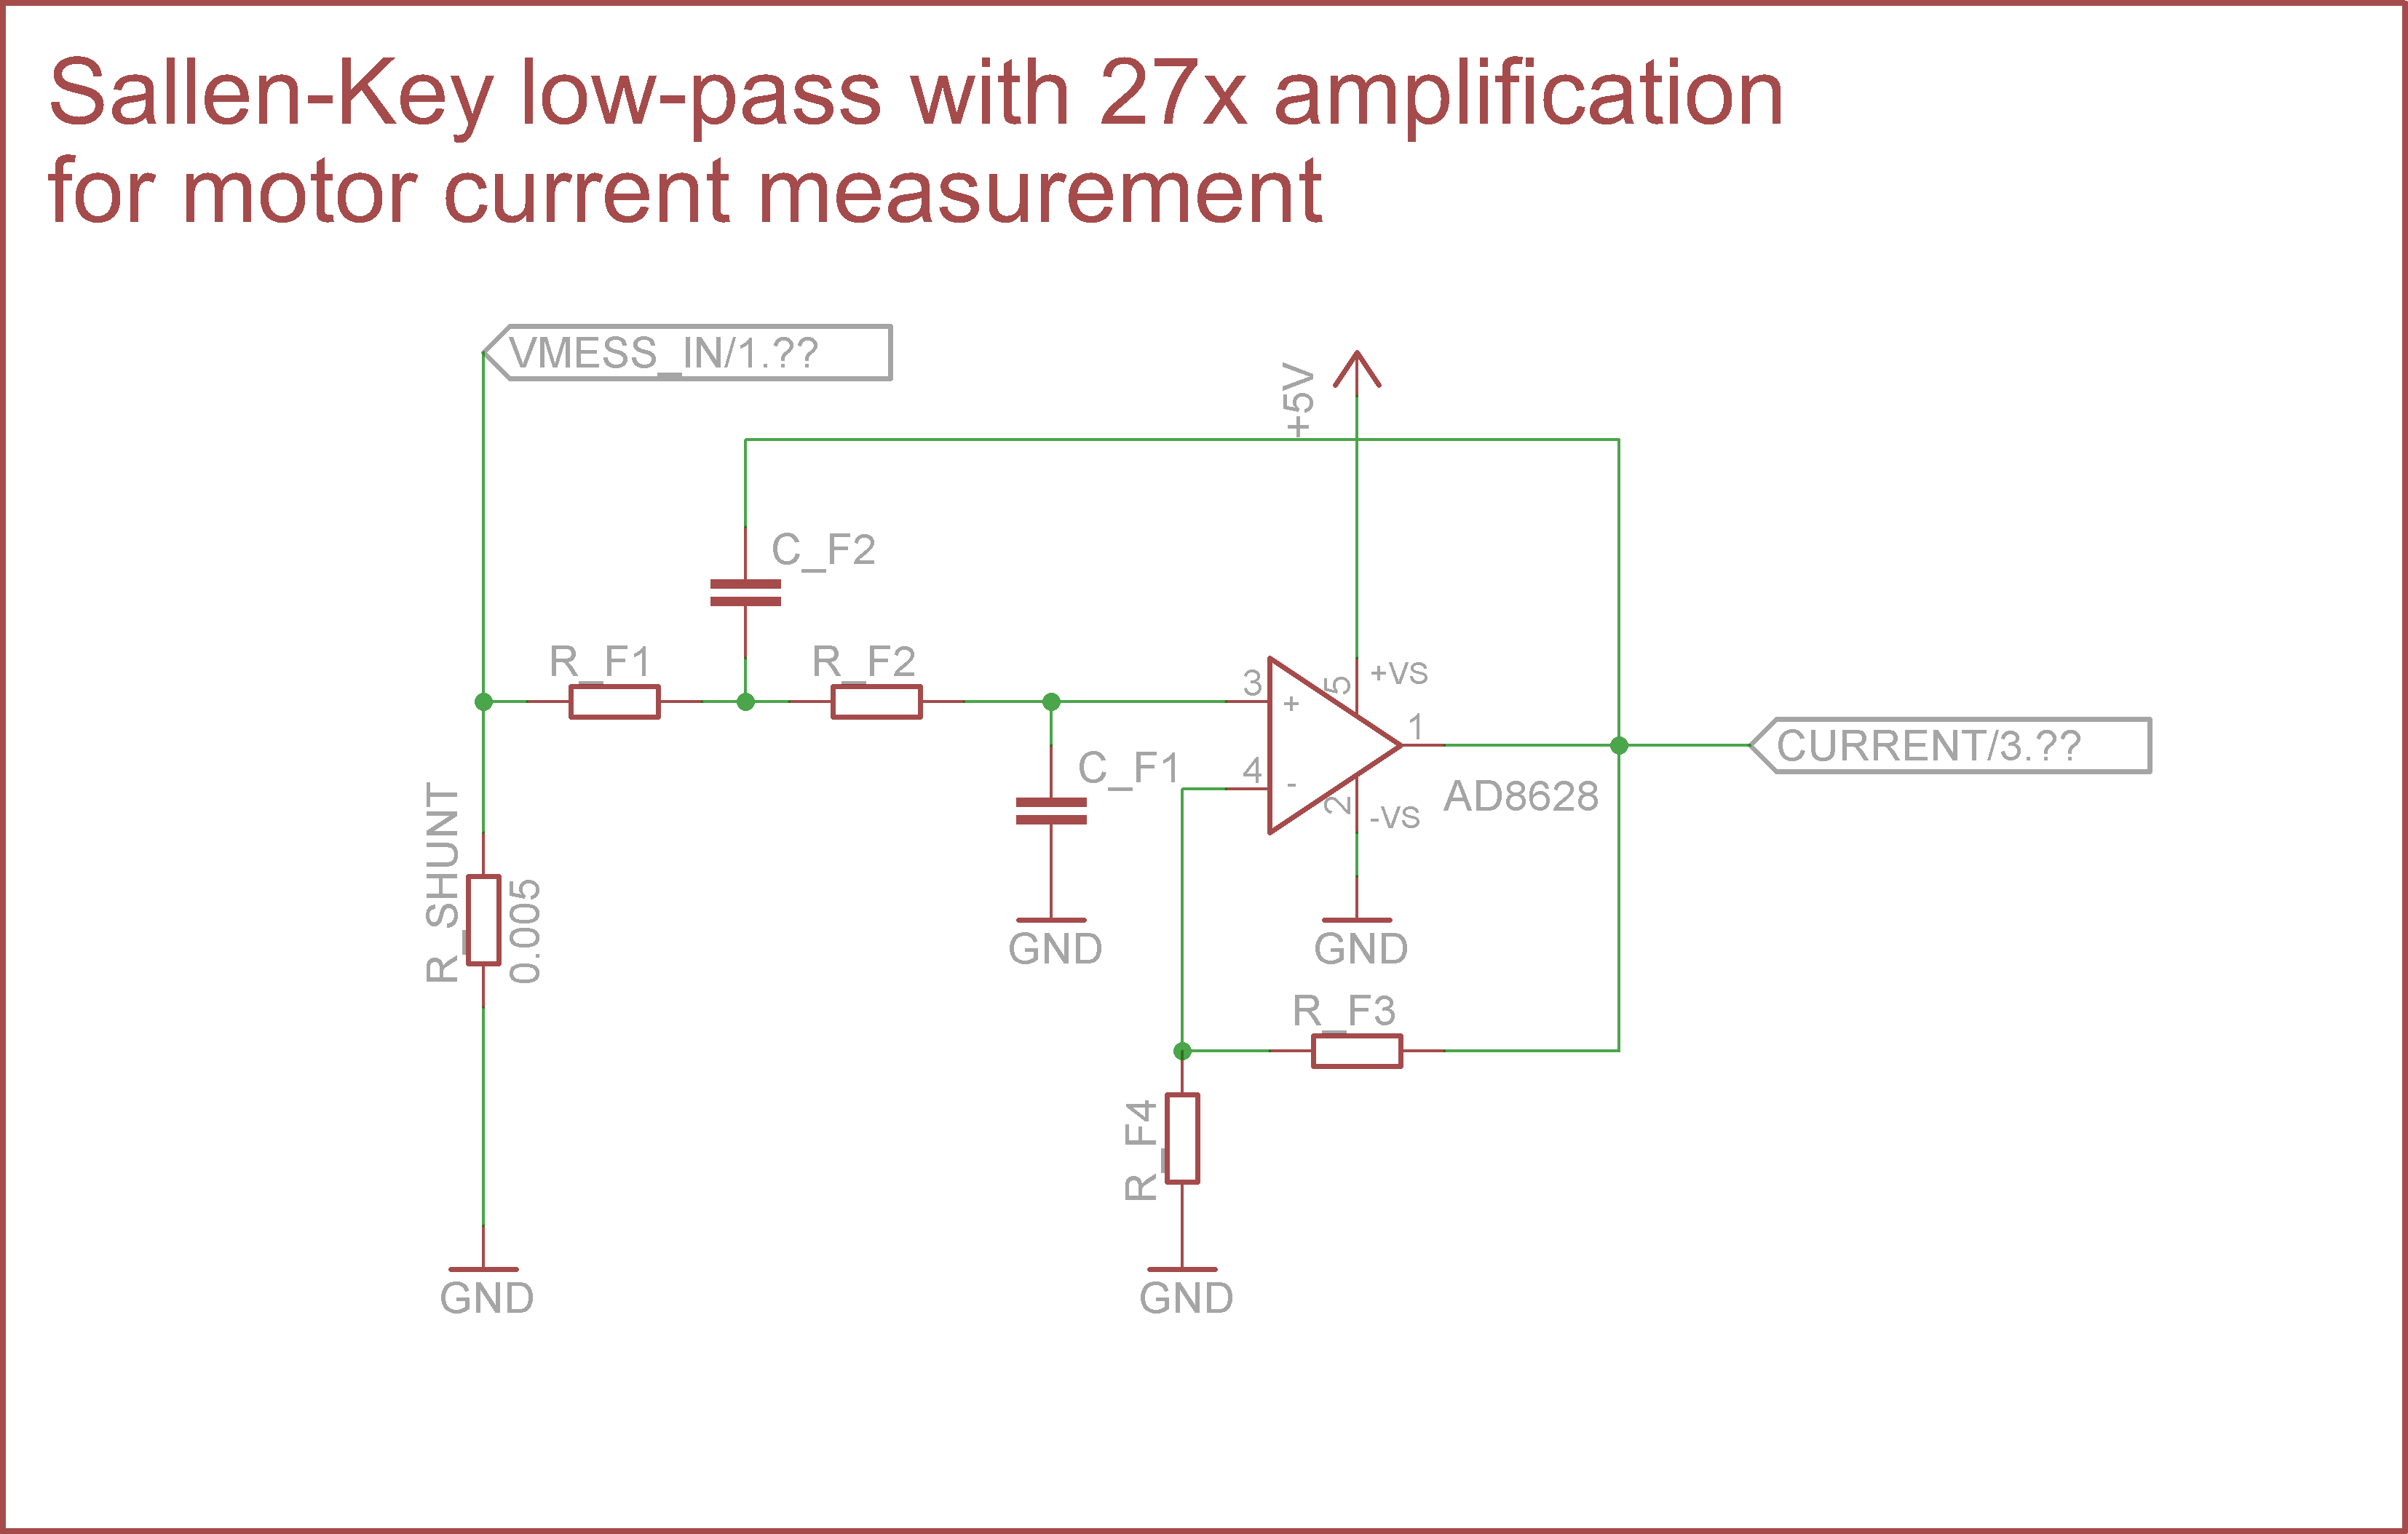
\includegraphics[width=.8\textwidth]{filter_schaltung.png}\\
\caption{Salle-Key Tiefpass mit Shunt}%
\label{fig:fschalt}
\end{figure}



\section{Dimensionierung des Verstärkers}

In bisherigen Rechnungen wurde ein maximaler Spannungsabfall von 100mV am Shunt errechnet. Da der Messbereich des voll ADC ausgenutzt werden soll,
ist es nötig das Messsignal zu verstärken. Hierzu wir ein Nichtinvertierender Verstärker benutzt. Da der Messbereich des ADC bis 5V reicht, wird hier eine 
50 fache Verstärkung angestrebt.

Für einem Nichtinvertierenden Verstärker ergibt sich dann:

\begin{align*}
v &= 1 + \frac{R_{F3}}{R_{F4}}\\
50 &= 1 + \frac{R_{F3}}{R_{F4}}\\
49\cdot R_{F4} &= R_{F3}
\end{align*}
\\
Wobei $R_{F4} = 47 k\Omega$ und $R_{F3} = 1 k\Omega$  gewählt werden, was eine Verstärkung von 48 ergibt.



\section{Anforderungen an den Filter}

\begin{figure}[H]
\centering
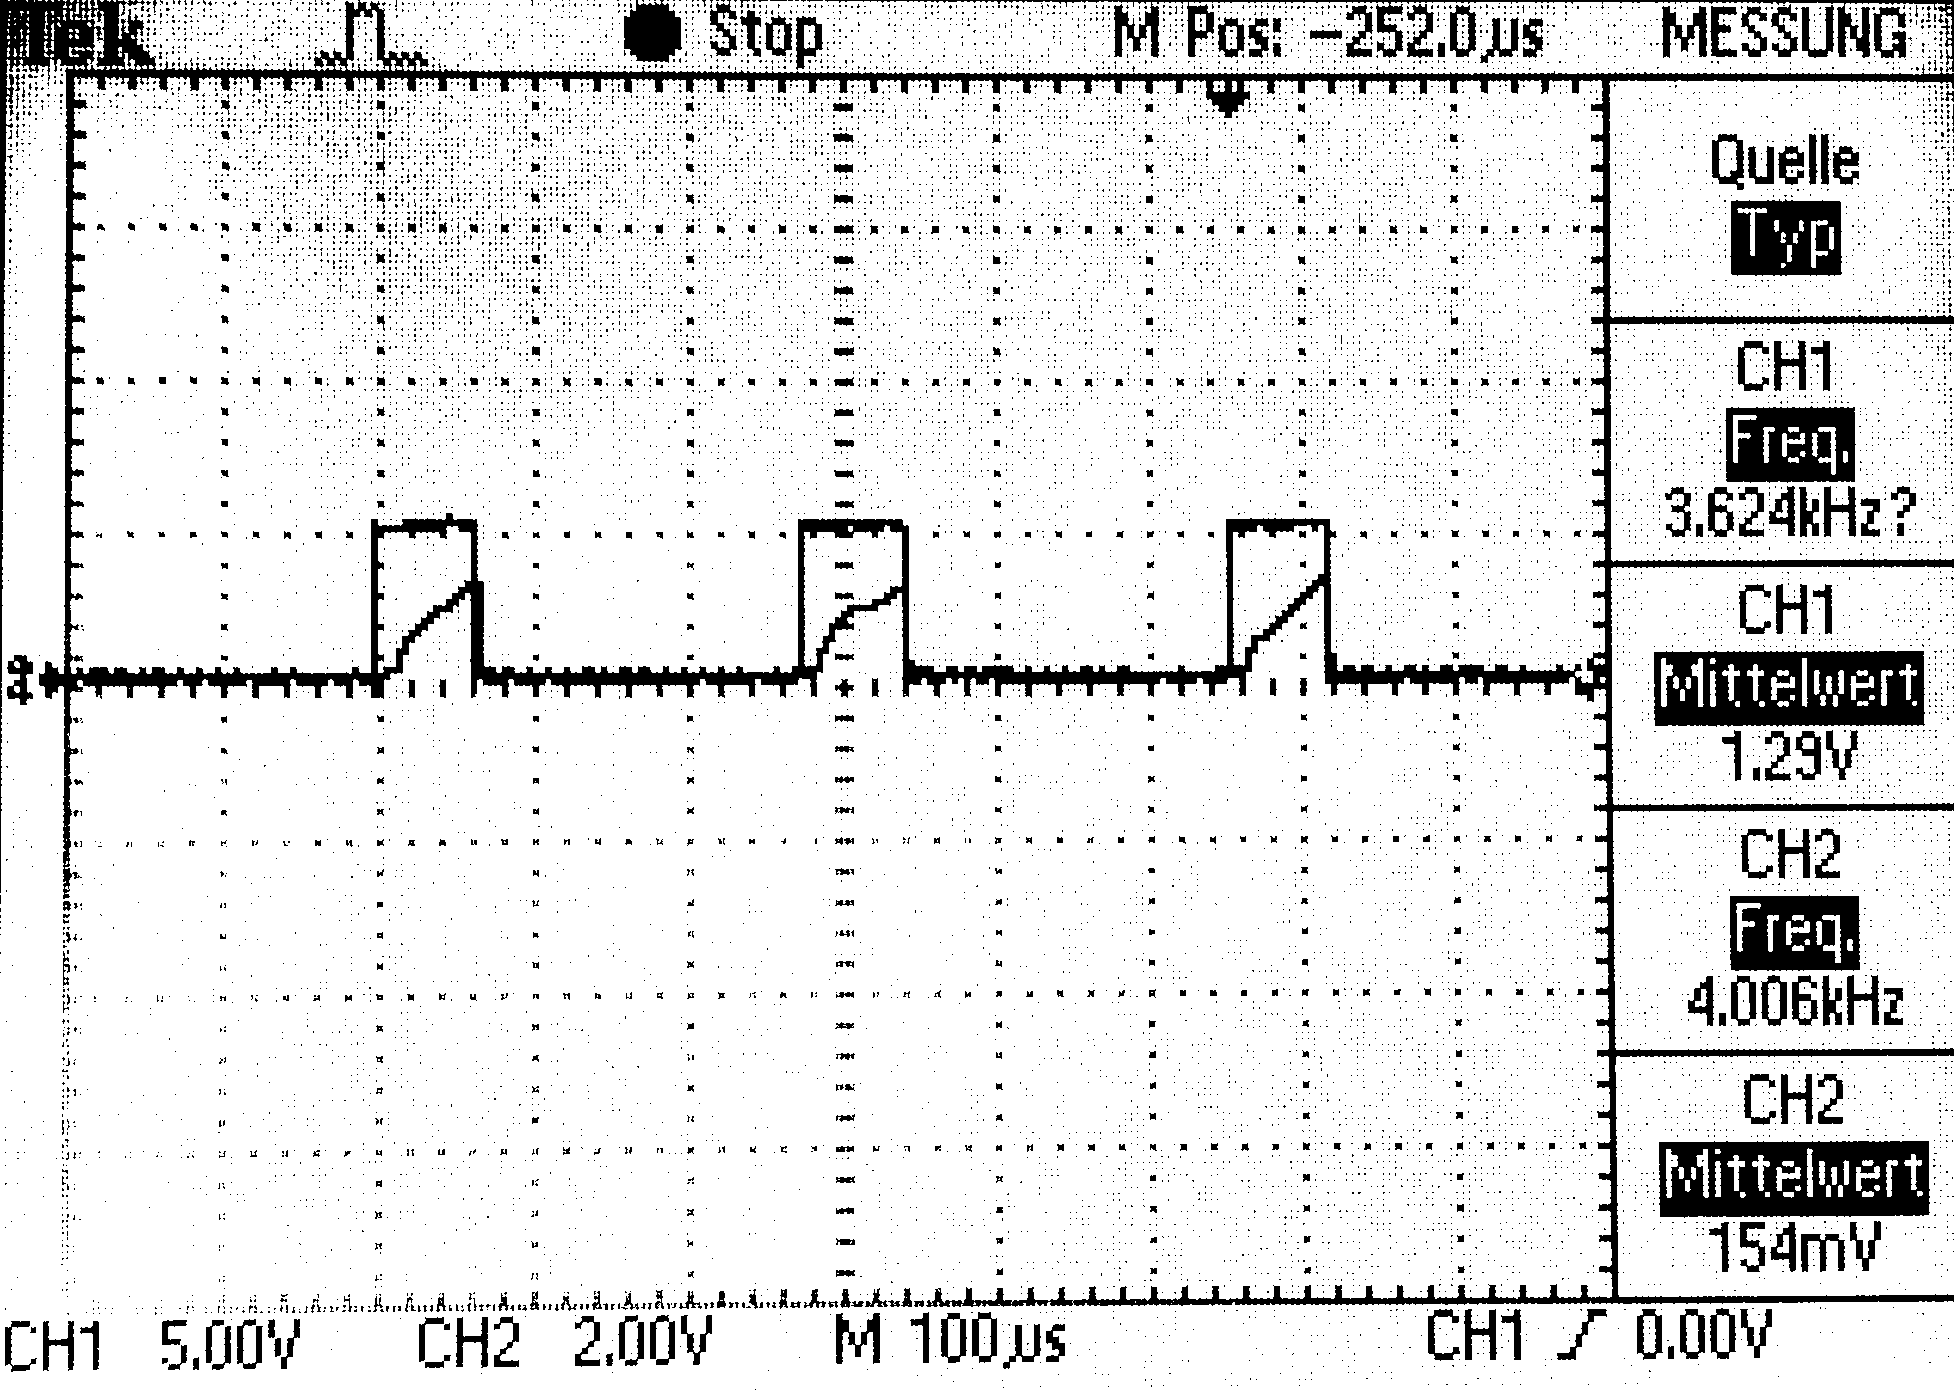
\includegraphics[width=.8\textwidth]{oszi.png}\\
\caption{Spannung am Shunt + PWM}%
\label{fig:pwm+i}
\end{figure}

Da dem Messsignal wie in Abbildung \ref{fig:pwm+i} zu erkennen, die PWM Frequenz zu Grunde liegt wird sich bei der Dimensionierung des Filters einer Idee nach \cite{Alter2008} bedient, nach der die maximale Amplitude des Ripple der Grundschwingung bei einem
Tastverhältnis von 0,5 entspricht. Die Amplitude der Grundschwingung ergibt sich aus dem ersten Koeffizienten der Fouerreihe einer Rechteckschwingung.
\begin{align}
A_1 = K\cdot \frac{1}{\pi}[\sin(\pi p)-\sin(2\pi(1-\frac{p}{2}))]
\label{eq:ripple}
\end{align}
Wobei p dem Tastverhältnis und K der maximale Amplitude des Ursprungsingals entspricht \cite{Alter2008}. K entspricht den errechneten 100mV multipliziert mit dem Verstärkungsfaktor 48, also 4,8V. p wird zu 0,5
angenommen. Mit (\ref{eq:ripple}) ergibt sich für die Amplitude der Grundschwingung $ A_1 = K\cdot \frac{2}{\pi} = 3,056V$. $A_1$ soll auf $ < 4,88mV$ gedämpft werden.
Als Sperrfrequenz $\Omega_s $ wird hier die PWM Frequenz angesetzt für $H(\omega=2\pi f_{PWM})$ gilt also:

\begin{align}
H(\omega=2\pi f_{PWM}) \le \frac{4,88mV}{3,056V} \mathop{\hat{=}} 20\cdot\log(\frac{4,88mV}{3,056V})= -55,9 dB
\label{eq:daempfung}
\end{align}

Da das Projekt möglichst kostensparend durchgeführt werden soll, also auch Bauteilsparend, wird an dieser Stelle von den üblichen Konventionen zur dimensionierung von Filtern abgewichen.
Statt eine fixe Grenzfreqeunz festzulegen und die benötigte Filterordnung zu bestimmen, wird die Filterordnung vorgegeben und die Grenzfrequenz variiert.

\section{Filterentwurf}

\subsection{Bestimmung des Filtertyps}

Des Filtertyp muss in Zweierlei hinblick bestimmt werden. Einmal im hinblick auf die Schaltung und seinem Frequenzgang.
Im groben gibt es 2 mögliche Tiefpassfilterschaltungen, den Sallen-Key Teifpass mit nicht invertierendem OPV und dem aktiven Tiefpass mit Mehrfachgegenkopplung 
(invertierender OPV). Der aktive Tiefpass mit Mehrfachgegenkopplung benötigt allerdings negative Spannungsniveaus die auf der Treiberplatine nicht zur
verfügung stehen, deshalb wird an dieser Stelle nur der Sallen-Key Teifpass behandelt.
Was den Frequenzgang angeht gibt es viele Filtercharakteristiken, eine Auswahl an haufig verwendeten Charakteristiken wird hier verglichen.

Der \emph{Butterworth}-Filter besitzt einen maximal flachen Verlauf des Frequenzganges im Durchlassbereich und eine monoton verlaufende Dämpfung im Sperrbereich.
Leider hat der Butterworth-Filter nur eine geringe Flankensteilheit im Sperrbereich. Ein Butterworth-Filter 1. Ordnung entspricht einen  einfachen RC-Filter.

Der \emph{Tschebyscheff}-Filter hat eine höhere Flankensteilheit als der Butterworth-Filter, allerdings entsteht beim Tschebyscheff-Filter Welligkeit im Durchlassbereich,
welche mit höherer Ordnung zunimmt. Durch die Welligkeit im Duchlassbereich würde ein zusätzlicher Ripple im Signal entstehen, weshalb der Tschebyscheff-Filter nicht
für den geforderten Filter geeignet ist 

Der \emph{Bessel-Filter} hat den Vorteil einer konstanten Gruppenlaufzeit, hat dafür aber eine noch geringere Flankensteilheit als der Butterworth-Filter.
Da eine konstante Gruppenlaufzeit für den geforderten Filter nicht von Vorteil ist, da das Endsignals einer Gleichspannung entsprechen sollte, ist der Butterworth-Filter
die bessere Wahl.


\begin{figure}[H]
\centering
\begin{tikzpicture}
	\draw[->,thick] (0,0) -- (7.5,0) node[right] {$f[\text{Hz}]$};
	\draw[->,thick] (0,0) -- (0,3.3) node[above] {$a[\text{dB}]$};
	\draw (0,2.5)node[left] {$a_{\text{min}}$} (-0.1,2.5)--(2.9,2.5);
	\draw (0,1)node[left] {$a_{\text{max}}$};
	\def \bsp{(0,1)--(1,1)--(1,2.4)--(1,2.4)--(0,2.4)}
	\draw (-0.1,1)--(1,1)--(1,2.4) (1,0)node[below] {$f_g$};
	\pattern[pattern=north east lines] \bsp;
	\draw[dashed] (1,1) -- (1,-0.1);
	\def \bsd{(3,0) -- (3,2.5) -- (7,2.5) -- (7,0)}
	\pattern[pattern=north east lines] \bsd;
	\draw (3,0)node[below] {$f_s$} -- (3,2.5) -- (7,2.5);

\end{tikzpicture}
\caption{Tiefpass Toleranzfeld}%
\label{fig:analog}
\end{figure}
Für unsere Schaltung wird ein Sallen Key Tiefpass 2. Ordnung entwurfen. Die PWM-Frequenz $f_{PWM}$ beträt 3,9kHz.
Die Sperrfrequenz entspreicht der PWM Frequenz, also der Frequenz unserer Grundschwingung. $\Omega$ entspricht der mit der Grenzfreqeunz 
normierten Frequenz $\Omega=\frac{f}{f_g}$. Nach (\ref{eq:daempfung}) ergibt sich für Abbildung \ref{fig:analog}
$f_s=f_{PWM}=3,9 kHz$, $a_{min}=55,9 dB$ und $a_{max}$ wird auf 3dB festgelegt.



\subsection{Butterworth}
\subsection{Bestimmung der Grenzfreqeunz}
\begin{align}
n \ge \frac{\log{\sqrt{\frac{e^{2a_{min}}-1}{e^{2a_{max}}-1}}}}{\log{\Omega_s}}
\label{eq:butterworth}
\end{align}
Die Filterordnung nach Butterworth wird nach (\ref{eq:butterworth}) bestimmt. Umgestellt nach $\Omega_s$ ergibt sich:

\begin{align}
\Omega_s \le  \left(\frac{e^{2a_{min}}-1}{e^{2a_{max}}-1}\right)^{\frac{1}{2n}}
\end{align}



Für die Berechnung der Sperrfrequenz $\Omega_s$ müssen  $a_{min}$ und $a_{max}$ in Neper umgrechnet werden. Wobei:
\begin{align*}
1 \text{dB} =  \frac{\ln{10}}{20}\text{Np} = 0,115129255 \text{Np}   
\end{align*}

Damit ergibt sich für $a_{min}=55,9 dB\cdot \frac{\ln{10}}{20}=6,45Np$ und für  $a_{max}=3 dB\cdot \frac{\ln{10}}{20}=0,345Np$. Die Filterordnung wird auf 2 festgelegt.
\begin{align}
\Omega_s \le  \left(\frac{e^{2\cdot6,45N }-1}{e^{2\cdot 0,345Np}-1}\right)^{\frac{1}{2n}}  = 35,8
\end{align}

Die Grenzfreqeunz $f_g$ ergibt sich jetzt aus:

\begin{align}
\frac{f_s}{\Omega_s} \le \frac{3,9kHz}{35,8} = 108,9Hz
\end{align}

\subsubsection{Filterentwurf}
Im voherigen Abschnitt wurde berechnet das die Grenzfreqeunz der Filters kleiner als 108,9Hz sein muss.
Im Folgenden wird nun ein Sallen-Key Filter 2. Ordnung mit einer Grenzfrequenz von 100Hz entwurfen.
Die genaue Wahl der Grenzfreqeunz ist hier nicht relevant da die realen Bauteile nicht in  allen Größen 
verfügbar sind und daher am Schluss variiert werden müssen, wodurch sich die Grenzfrequen des Filters leicht ändert.


\subsubsection{Finaler Entwurf}



Betrachetn wir das Polstellen-Nullstellendiagramm eines Butterworth Filters 2. Ordnung, wie in Abbildung [\ref{fig:filter_polnul}]


\begin{figure}[H]
\centering
\begin{tikzpicture}
	\draw[->,thick] (-3,0) -- (3,0) node[right] {$\text{Re}$};
	\draw[->,thick] (0,-3) -- (0,3) node[above] {$\text{Im}$};
	\draw[dashed,red,very thin] (-3,2) -- (3,2);
	\draw[dashed,red,very thin] (-3,-2) -- (3,-2);
	\draw[dashed,red,very thin] (2,-3) -- (2,3);
	\draw[dashed,red,very thin] (-2,-3) -- (-2,3);
	\draw[dashed,blue,very thin] (0,0) circle (2);
	\coordinate (x) at (225:2); 
	\coordinate (y) at (135:2);
	\draw[very thin] (0,0) -- (y);
	\draw[red,thick] (x) -- +(0.1,0.1)  (x) -- +(-0.1,-0.1) (x) -- +(0.1,-0.1) (x) -- +(-0.1,0.1);
	\draw[red,thick] (y) -- +(0.1,0.1)  (y) -- +(-0.1,-0.1) (y) -- +(0.1,-0.1) (y) -- +(-0.1,0.1);
	\draw (2,0)node[below] {$1$};
	\draw (-2,0)node[below] {$-1$};
	\draw (0,2)node[left] {$1$};
	\draw (0,-2)node[left] {$-1$};
	\draw (0,-2)node[left] {$-1$};
	\draw (0,0) (135:1cm) arc (135:180:1cm);
	\draw (-0.6,0.3)node {$\delta$};
\end{tikzpicture}
\caption{Polstellen-Nullstellendiagramm, Butterworth 2. Ordnung}
\label{fig:filter_polnul}
\end{figure}



Charakteristisch für den Butterworthfilter ist das sich die Polstellen auf einer Kreisbahn befinden. Auf die Grenzfreqeunz normiert hat dieser beim Butterworthfilter den Radius
eins. Bei einem Butterworth 2. Ordnung befinden sie sich genau bei $\delta=45^\circ$. Das Interessante am Polstellen-Nullstellendiagramm ist, dass sich Polfrequenz $\Omega_P$ und 
Polgüte $Q_P$ einfach ablesen lassen. Die Polfrequenz $\Omega_P$ ist der Betrag der normierten Polstelle, welcher beim Butterworth-Filter immer eins ist.
Die Polgüte ist abhängig von $\delta$ und ergibt sich zu: $Q_P=\frac{1}{2\cos{\delta}}$. Für unseren Butterworthfilter ergeben sich also $Q_P=0,707$ und $\Omega_P=1$



Bet

Betrachten wir deie Übertragungsfunktion eines Sallen-key Tiefpasses 2. Ordnung:

\begin{align*}
A(P)&=\frac{A_0}{1+\omega_g (R_2 C_2 + R_1 C_2 + R_1 C_2(1-A_0))P + \omega_g^2R_1 R_2 C_1C_2P^2}
\end{align*}

mit
\begin{align*}
A_0=1+\frac{R_6}{R_5}
\end{align*}


Die Bauteilwerte erhält man durch einen Koeffizientenvergleich mit der entnormierten
Übertragungsfunktion ($P=\frac{s}{\omega}$) eines Tiefpasses zweiter Ordnung:

\begin{align*}
A(P)&=\frac{A_0}{1+\frac{1}{\omega_g\Omega_PQ_P}s+\frac{1}{\omega_g^2\Omega_P^2}s^2}
\end{align*}

Die Auflösung des Vergleiches ist mit vielen Mathematischen umformungen verbunden, deswegen wird hier auf eine
externe Quelle verwiesen \cite[Seite: 102]{Krucker2000}.
Nach dem Koeffizientenvergleich ergibt sich

\begin{align*}
C_1&<\frac{C_2\cdot(1+4Q^2_P(A_0-1))}{4Q^2_P}\\
R_1&=\frac{1}{2\omega_g\Omega_PQ_P} \cdot \frac{C_2\pm\sqrt{C_2^2-4Q^2_PC_2(C_1+C2(1-A_0))}}{C_2(C_1-C_2(1-A_0))}   \\
R_2&=\frac{1}{2\omega_g\Omega_PQ_P} \cdot \frac{C_2\pm\sqrt{C_2^2-4Q^2_PC_2(C_1+C2(1-A_0))}}{C_1C_2}  \\
Q_p&=\frac{\sqrt{R_1R_2C_1C_2}}{C1(R_1+R_2)+R_1C_2(1-A_0)}\\
\Omega_p&=\frac{1}{\omega_g\sqrt{R_1R_2C_1C_2}}
\end{align*}

Dabei sind immernur die positiven, reellen Lösungen zu verwenden. Schließlich git es in der Realität keinen negativen Wiederstand, leider.


\subsubsection{Bestimmung der Bauteilwerte}


$Q_P=0,707$ und $\Omega_P=1$, $A_0=48$, $\omega_g = 100Hz$
$A_0$ ist die Gleichspannungsverstärkung, sie beschreibt den gewünchten Verstärkungsfaktor der Bereits in einem voherigen
Abschnitt mit 48 bestimmt wurde. Die Berechnungen wurden mit Hilfe eines Python-Scriptes ausgeführt, dabei wurden verschiedenne
Konfigurationen durchgerechnet. Hautpsächlich wurde dabei darauf geachtet, dass sich der Filter mit den vor Ort vorhandennen SMD-Bauteilen
aufgebaut werden kann.

In den Berechnungen viel auf, dass bei steigender größe der Kondensatoren die Größe der Wiederstände sinkt. Da Wiederstände auch in großen Größen vorhanden waren,
Wurde für den frei wählbaren $C_2$ ein kleiner Wert von 82nF gewählt.

\begin{align*}
C_1&<\frac{C_2\cdot(1+4\cdot0.707^2_P(48-1))}{4\cdot0.707^2}\\
C_1&<3.90µF\\
\end{align*}

$C_1$ soll nur kleiner sein als 3.90µF und wird ebenfalls auf 82nF gesetzt.

\begin{align*}
R_1&=\frac{1}{2\cdot100Hz\cdot0,707} \cdot \frac{82nF\pm\sqrt{82nF^2-4\cdot0.707^2\cdot82nF(82nF+82nF(1-48))}}{82nF(82nF-82nF(1-48))}\\
R_1&=[-3176\Omega,2579\Omega]
\end{align*}


\begin{align*}
R_2&=\frac{1}{2\cdot100Hz\cdot0,707} \cdot \frac{82nF\pm\sqrt{82nF^2-4\cdot0.707^2\cdot82nF(82nF+82nF(1-48))}}{82nF^2}\\
R_2&=[146079\Omega,-118626\Omega]
\end{align*}

Da natürlich nur positive Werte genutzt werden können, hat ergeben sich die Bauteilwerte nun zu:
\begin{align*}
C_1&=82nF\\
C_2&=82nF\\
R_1&=2579\Omega\\
R_2&=146079\Omega
\end{align*}

%%Verstärkung: 33,6dB gewünscht:
%%20*log(1/48)=-33,6

%%dämpfung bei 3,9Khz = 30,7dB
%% 33,6+30,1 =63,7 gewüncht: 55,9
%% Grenzfreqeunz = 100Hz (-3db)
\begin{gnuplot}[terminal=pdf]
  set nokey 
  set xrange [10:3900]
  set xlabel 'Frequenz in [Hz]'
  set ylabel 'Verstärkung in [dB]'
  set logscale x 10
  plot 'Simulation/Filter_original_frequenzgang.csv' with line
\end{gnuplot}






%%Verstärkung: 33,6dB gewünscht:
%%20*log(1/48)=-33,6

%%dämpfung bei 3,9Khz = 30,7dB
%% 33,6+30,7 =64,3 gewüncht: 55,9
%% Grenzfreqeunz = 104Hz (-3db)
\begin{gnuplot}[terminal=pdf]
  set nokey 
  set xrange [10:3900]
  set xlabel 'Frequenz in [Hz]'
  set ylabel 'Verstärkung in [dB]'
  set logscale x 10
  plot 'Simulation/Filter_real_frequenzgang.csv' with line
\end{gnuplot}



\begin{gnuplot}[terminal=pdf]
  set nokey 
  set yrange [0:3]
  set xlabel 'Zeit in [s]'
  set ylabel 'Spannung in [V]'
  plot 'Simulation/Filter_real_time.csv' with line
\end{gnuplot}


%% Ripple: 0,003358
%% zu hoher Spannungswert durch Steig und Fallzeiten im low bereich des Rechtecksignals
\begin{gnuplot}[terminal=pdf]
  set nokey 
  set xrange [0.03:0.04]
  set yrange [2.62:2.66]
  set xlabel 'Zeit in [s]'
  set ylabel 'Spannung in [V]'
  plot 'Simulation/Filter_real_time.csv' with line
\end{gnuplot}

\chapter{Software}

Die Software besteht im Grunde aus zwei Teilen, zum einem der Firmware auf dem \textmu Controller zum anderem aus der Software auf dem NUC, welche die Daten vom \textmu Controller ausließt und über ROS publisht.
In den Folgenden Abschnitten werden Erst die Beiden Softwareteile erläutert, dann wird das Übertragungsprotokoll veranschaulicht.


\section{Software auf dem \textmu Controller}
Die Software auf dem \textmu Controller ist vollständig in C++ geschrieben. Eine volständige Dokumentation der Software ist als Doxygen Dokument verfügbar.


\section{Client Programm auf der Recheneinheit}
Das Client Programm im folgenden SerialNode genannt 
Im erten Schritt wurde hier ein Python Programm genutzt, welches jedoch einen Nachteil mit sich bringt. Da das ansprechen der seriellen Schnitstelle unter pyserial sehr hohe CPU-Last mit sich bringt.
Da die so verschwendete Rechenleistung für andere Aufgaben benötigt wird und auch energieeffizienz ein wichtiges Kriterium ist, Wurde das Programm erneut in C++ implementiert. Unter verwendung der Systemaufrufe von 
Poll konnte das abfragen der seriellen Schnitstelle auf Systemebene ausgeführt werden, was die effizeinz stark verbessert. Während die Python Implementierung einen CPU-Kern zu 100\%
auslastete liegt die C++ Implementierung im unteren einstelligen Bereich.


\section{Übertragungsprotokoll}
Da die Übertragung der Daten via ROS-Serial im ersten Prototypen zu vielen Problemen geführt hat, wurde ien neues Übertragungsprotokoll entwickelt.
Dabei wurde auf Fehlertolleranz niedrigen Ressourcenverbrauch geachtet. Der Datendurchsatz muss hier ausreichend sein um alle Daten stabil mit 100Hz
übertragen zu können.


Der Grundlegende Ablauf der Datenübertragung ist in den Abbildungen [\ref{fig:uC_read}] und [\ref{fig:uC_write}] zu sehen.



\begin{figure}[ht]
\centering
\includegraphics[page=1,width=.8\textwidth]{graph/read.pdf} 
\caption{Lese Daten}
\label{fig:uC_read}
\end{figure}


\begin{figure}[ht]
\centering
\includegraphics[page=1,width=.8\textwidth]{graph/write.pdf} 
\caption{Schreibe Daten}
\label{fig:uC_write}
\end{figure}



\chapter{Evaluierung}

\section{Motoransteuerung}

\section{Strommessung}

\section{Stromverbrauch}

\section{Infrarotsensoren}

\section{Inertialsensor}

\section{Zeitverhalten der seriellen Verbindung}

\chapter{Ausblick und Fazit}

Im Rahmen dieser Arbeit wurde eine Treiberplatine für das OttoCar geschaffen, ausgehend von einem Anfangsbestand von Komponenten sollte die Platine, diversen Anforderungen genügen.
Die Anforderungen umfassten dabei die Ansteuerung des Motors und des Servomotors, welche erfolgreich umgesetzt wurden, und zuverlässig ihren Dienst verrichten.
Auch die Sharp GP2D Sensoren konnten erfolgreich in das System integriert werden....................................................Evaluierung Sensorqualität
Die benötigte Beleuchtung wurde durch einen LED-Streifen mit WS2812 Controllern umgesetzt, welche durch ihre Bauart eine einfache Integration in das Auto ermöglichen.
Da diese als RGB-LEDs ausgeführt sind Übertreffen sie die Anforderungen sogar, da sie nahezu jede mögliche Farbe Annehmen können. Innerhalb der Software können diese einzeln Angesteuert
werden und so zu Fehlerdiagnose genutzt werden. Bei der Integration des Sparkfun Inertialsensors traten Probleme mit dem Magnetometer auf, welche im Nachhinein nur provisorisch abgemildert werden konnten.
Trotz diese Probleme kann der Inertialsensor erfolgreich ???????????????? zur Inertialnavigation eingesetzt werden %%%%%%%%\cite{Martins_arbeit}}

Die Auslegung der 5V Stromversorgung kann ebenfalls als Erfolg gewertet werden, der Regler schafft es trotz enormer Schwankungen der Betriebsspannung die Spannung, bis auf minimale Störungen
stabil zu halten, so dass es zu keiner Störung der Sensormesswerte kommt. Die Odometrie konnte die Anforderungen leider nicht vollständig erfüllen, da nur eine Wegmessung nach vorne möglich ist.
Die Qualität der Geschwindigkeitsangabe ist dafür auch bei Mittleren Geschwindigkeiten bis \SI{2}{\metre\per\second} auch in Kurven gut brauchbar. Durch die Fusion, der
Inertialsensorik und Odometrie konnte ein Inertialnavigationssystem
%%%%%%%%\cite{Martins_arbeit}}
entwickelt werden, welche eine gute????????????????? Aussage über die Postion des Autos machen kann.

Als großer Erfolg, kann die Energieeffizeins des Systems gewertet werden! 
In zuk+nftigen entwicklingenn sollte die Leistungselkektronik jedoch von ser Sensorkmgetrennt werden, um Störungen zu vermeiden

% \item nötige Elektonik zur Motoransteuerung (vor und Rückwärts)
% \item Anschluss und Steuerung für einen Servomotor
% \item Anschlusse und Steuerung für die nötige Beleuchtung
% \item Anschlüsse für die Sharp GP2D Sensorn
% \item Integration des Sparkfun Inertialsensors
% \item Leistungsfähige Stromversorgung

\chapter{Ausblick}


\listoffigures

\bibliography{BIB}{}
\bibliographystyle{alpha}

\end{document}